%%%%%%%%%%%%%%%%%%%%%%%%%%%%%%%%%%%%%%%%%%%%%%%%%%%%%%%%%%%%%%%%%%%%%%%%
% Plantilla TFG/TFM
% Escuela Politécnica Superior de la Universidad de Alicante
% Realizado por: Jose Manuel Requena Plens
% Contacto: info@jmrplens.com / Telegram:@jmrplens
%%%%%%%%%%%%%%%%%%%%%%%%%%%%%%%%%%%%%%%%%%%%%%%%%%%%%%%%%%%%%%%%%%%%%%%%

\chapter{Desarrollo}
\label{desarrollo}
Este apartado va a ser el que contenga los detalles sobre la implementación de la aplicación, tanto frontend como backend, mostrando código, capturas de la misma y acceso a dos vídeos de las funcionalidades de una forma resumida.
\section{Funciones}
Una de las primeras cosas que se hizo antes de empezar el desarrollo, fue una tormenta de ideas para decidir las funcionalidades y el alcance de éstas en el proyecto; estableciendo de esta manera un producto mínimo viable que entregar.
\vspace{1em}
\par Las funcionalidades que se decidió entregar como mínimo fuero:
\begin{itemize}
    \item Gestión de usuarios: Capacidad de crear usuarios, activarlos y desactivarlos, cambiarles la contraseña y atomizar los roles y permisos.
    \item Gestión de almacenes: Capacidad de crear y editar almacenes, los almacenes son la entidad más alta de la aplicación, sólo comparten súper administradores entre sí.
    \item Leer EAN por hardware: Capacidad de leer los códigos de barras de los productos mediante un lector específico o la webcam.
    \item Recepción de pedidos: Capacidad de recibir pedidos de productos con limitaciones muy concretas configuradas en la creación del producto, limitar al máximo la capacidad humana de fallar en estas limitaciones.
    \item Recepción del pedido restricciones familiares: Las familias tienen restricciones de cuánto y cuántas veces pueden consumir productos del banco de alimentos. Capacidad automática de gestionar estas limitaciones, con la mínima interacción humana.
    \item Gestión de productos: Capacidad para añadir y editar productos. Éstos productos deben poder tener un EAN asociado y solicitar información pública de OpenFoodFacts para añadir información nutricional a su ficha. Hay bancos de alimentos que cuentan con personal sanitario al que puede resultarle útil tener esta información a mano.
    \item Facturación y caja: Capacidad de cobrar facturas y buscarlas por rango de fechas para consultas posteriores.
    \item Impresión de facturas: Capacidad de ver las facturas maquetadas para imprimirlas fácilmente.
    \item Expedición de pedidos: Capacidad de ver qué pedidos están pendientes de despachar para que almacén pueda prepararlos con antelación.
    \item Dashboard con gráficas: Capacidad de ver intuitivamente datos relevantes que faciliten al personal la previsión de trabajo.
\end{itemize}
\vspace{1em}
\par Además de ciertas solicitudes y cambios puntuales en la forma en la que la aplicación iba funcionando, que entraban dentro de la prevención de riesgos y las estimaciones; se solicitaron funcionalidades nuevas casi a última hora. Como la gestión temporal fue un éxito y se iba holgado en tiempo, se aceptaron las solicitudes y se implementaron.
\vspace{1em}
\par La nuevas funcionalidades fueron:
\begin{itemize}
    \item Anonimizar facturas: Capacidad de desvincular familias y facturas, además de la LOPD, Cáritas manda, y al no tener, en el banco de alimentos, muy clara la política de datos personales; se solicitó una funcionalidad capaz de anonimizar facturas de forma permanente, por si acaso.
    \item Productos de higiene especial: Capacidad de configurar ciertos productos como especiales, éstos productos podrían impactar o no en las limitaciones de la familia, pudiendo ser ésta (en el proceso de pedido) la que decida si quiere que éstos productos afectasen a los límites de las facturas de su expediente, o no.
\end{itemize}

\section{Pantallas}
Una vez definidas las funcionalidades que deberá atender la aplicación, se pasó a organizar las diferentes pantallas que tendrá. La gama de colores usadas se dejaron a discreción del tema por defecto de Angular Material, debido a la falta de conocimientos de diseño. El menú usa escalas de grises por decisión estética personal.
\vspace{1em}
\par Los colores permiten una clara diferenciación de qué implicaciones tendrán las acciones asociadas al uso de éstos botones. Listémoslos:
\begin{itemize}
    \item Color azul:
    \begin{itemize}
        \item Acciones que activan, aceptan o navegan a subsecciones o funcionalidades relacionadas.
        \item Combinaciones entre vacíos con iconos o textos azules, o rellenos azules con contenido blanco.
    \end{itemize}
    \item Color rojo:
    \begin{itemize}
        \item Acciones que desactivan, cancelan, vacían datos o navegan a secciones anteriores.
        \item Combinaciones entre vacíos con iconos o textos rojos, o rellenos rojos con contenido blanco.
        \item Mensajes relacionados con errores o acciones que son irreversibles.
    \end{itemize}
    \item Color verde:
    \begin{itemize}
        \item Mensajes relacionados con acciones realizadas correctamente por el servidor.
    \end{itemize}
\end{itemize}
\begin{figure}[h]
\centering
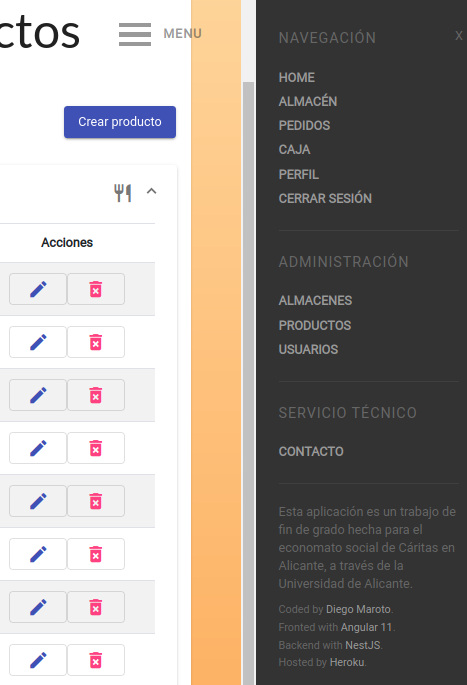
\includegraphics[scale=0.8]{archivos/decision_cromatica.png}
\caption{Ejemplo colores de la aplicación}
\label{fig:decision_cromatica}
\end{figure}
\clearpage

\subsection{Login}
\begin{figure}[h]
\centering
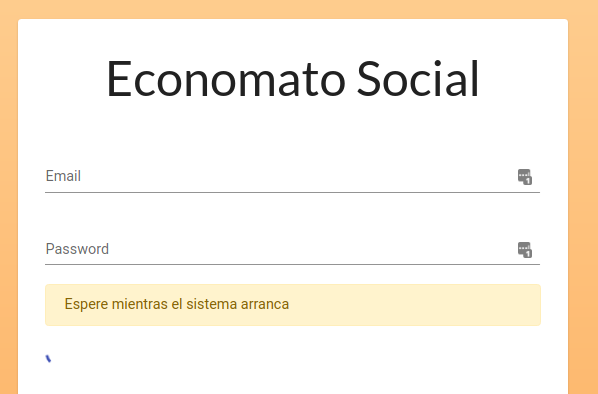
\includegraphics[scale=0.7]{archivos/login-esperando-backend.png}
\caption{Login esperando respuesta del backend}
\label{fig:login_esperando_backend}
\end{figure}
\vspace{1em}
\par En esta figura se muestra cómo el frontend, para evitar frustración del usuario, avisa de que el backend aún tienen que arrancar y debe esperar. Esto es dado por tener el frontend y el backend alojados de forma independiente y habiendo usando heroku como hosting.
\vspace{1em}
\par En heroku cuando la aplicación no recibe peticiones en 5 minutos, muere, esto hace que la siguiente petición tarde más en responder, dado que debe arrancar el sistema; Pudiendo tardar entre 20 segundos y un minuto. Esta pantalla es la que el primer voluntario que acceda a la aplicación verá cada día.
\clearpage
\begin{figure}[h]
\centering
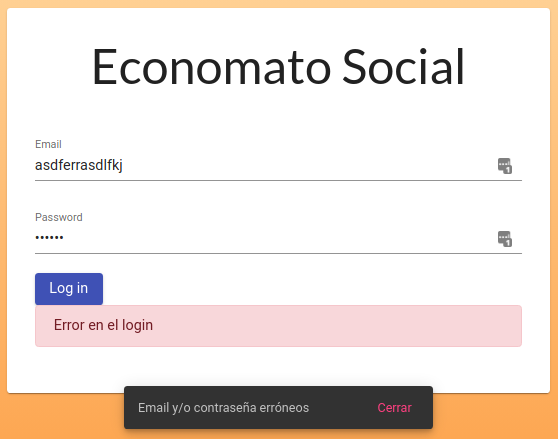
\includegraphics[scale=0.7]{archivos/login-credenciales-incorrectas.png}
\caption{Login error credenciales}
\label{fig:login_error_credenciales}
\end{figure}
\vspace{1em}
\par Este sería el comportamiento de un login incorrecto. Una posible mejora, que sería crítica en caso de ataque, sería añadir un captcha y/o un rate limiter a este tipo de vectores de ataque.
\vspace{1em}
\par Propuse añadir un rate limiter a este endpoint, dado que es el único que no requiere un jwt debidamente firmado y en vigor, pero como habían tareas más acuciantes pendientes y llegaron otras nuevas, se decidió dejar para una versión posterior.
\clearpage
\begin{figure}[h]
\centering
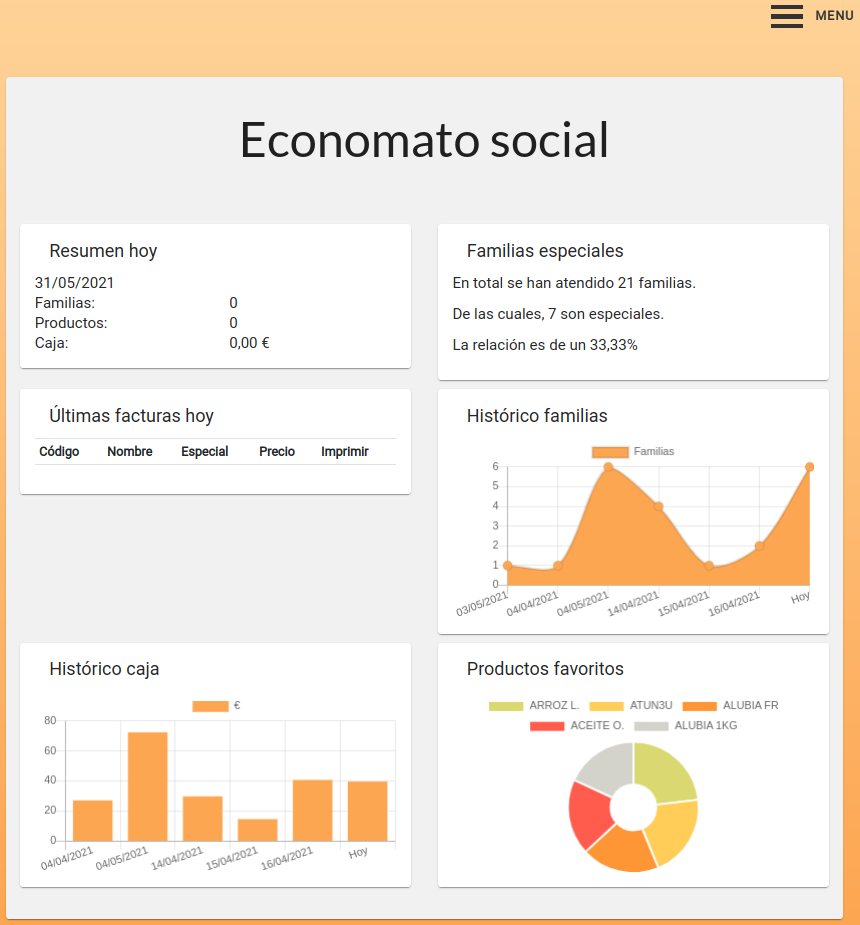
\includegraphics[scale=0.47]{archivos/dashboard.png}
\caption{Dashboard}
\label{fig:dashboard}
\end{figure}
\vspace{1em}
\par Tras un login correcto, se muestra el dashboard.
\clearpage
\subsection{Pedidos}
La sección de pedidos es un stepper, es decir, una única página que se mueve adelante y atrás de forma dinámica y a discreción del usuario y con alguna automatización. Esta sección es la que crea las facturas y para ello se obliga a que el voluntario pase por 3 subsecciones:
\begin{itemize}
    \item Búsqueda de la familia que está atendiendo, para que el sistema tenga en cuenta su histórico del mes en las restricciones de la compra
    \item La gestión de los productos que desea adquirir
    \item Resumen del pedido y generación de la factura
\end{itemize}
\vspace{1em}
\par Después de generar la factura, ésta se abre en una pestaña nueva; maquetada de forma limpia e independiente y lista para imprimir.
\begin{figure}[h]
\centering
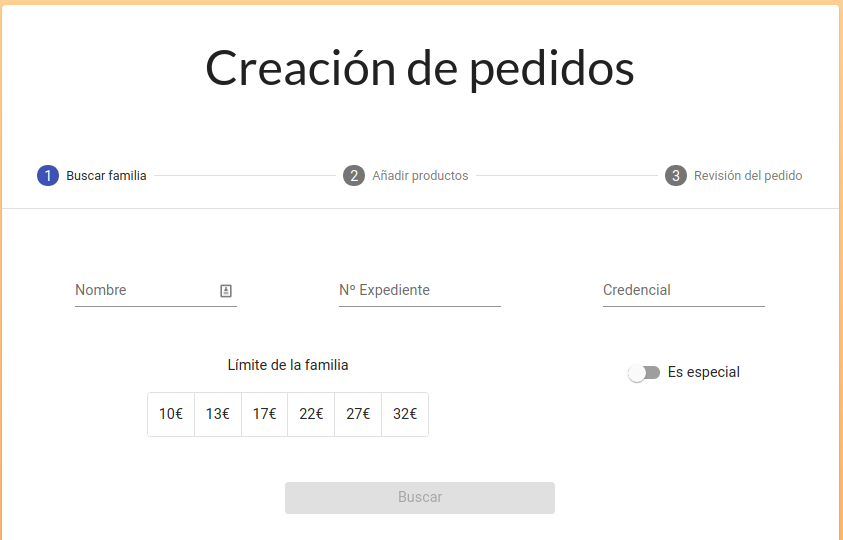
\includegraphics[scale=0.47]{archivos/pedidos-step1.png}
\caption{Pedidos: Step 1 - Búsqueda de familia}
\label{fig:pedidos_step1}
\end{figure}
\begin{figure}[h]
\centering
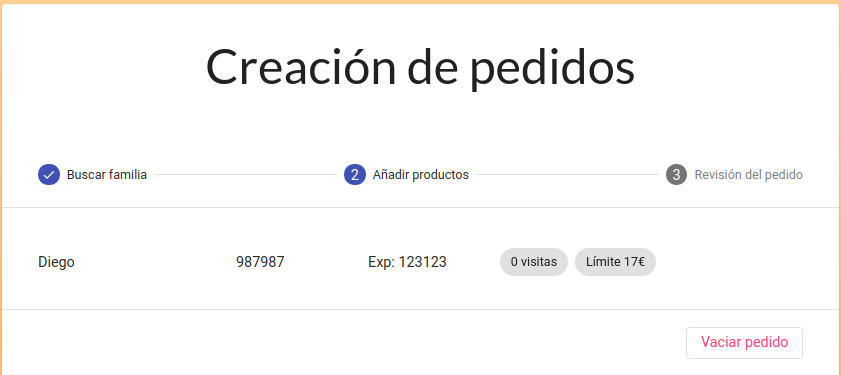
\includegraphics[scale=0.47]{archivos/pedidos-step2.png}
\caption{Pedidos: Step 2 - Resumen familia en gestión del pedido}
\label{fig:pedidos_step2_1}
\end{figure}
\begin{figure}[h]
\centering
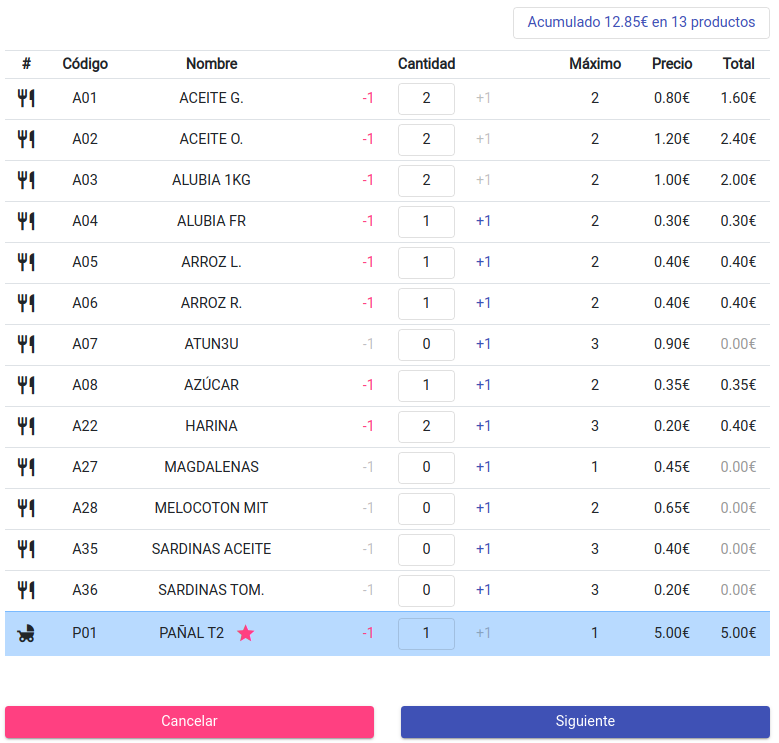
\includegraphics[scale=0.5]{archivos/pedidos-productos-resumen-botones.png}
\caption{Pedidos: Step 2 - Gestión del pedido}
\label{fig:pedidos_step2_2}
\end{figure}
\clearpage
\begin{figure}[h]
\centering
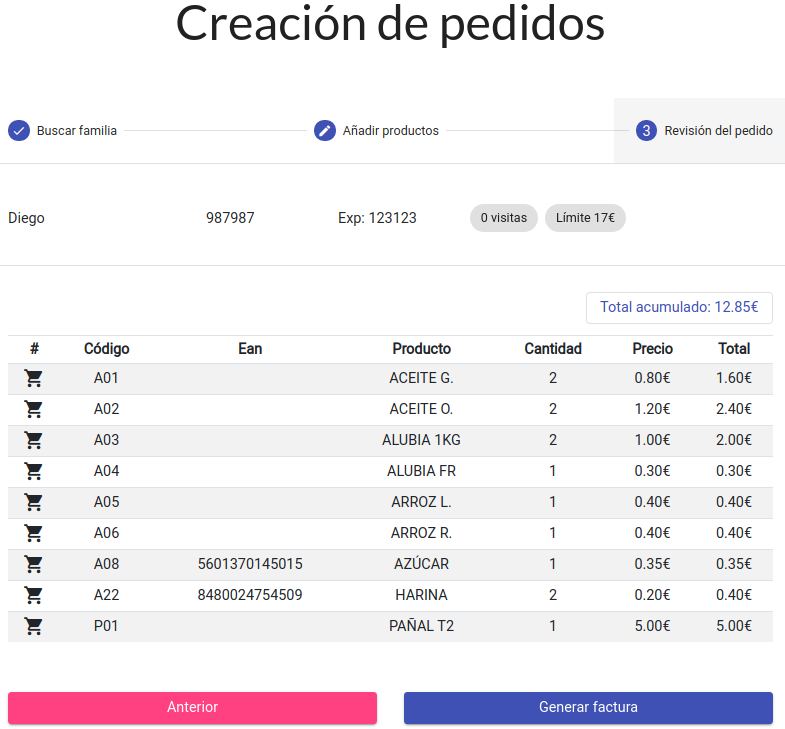
\includegraphics[scale=0.47]{archivos/pedidios-step3.png}
\caption{Pedidos: Step 3 - Resumen del pedido}
\label{fig:pedidos_step3}
\end{figure}
\clearpage
\begin{figure}[h]
\centering
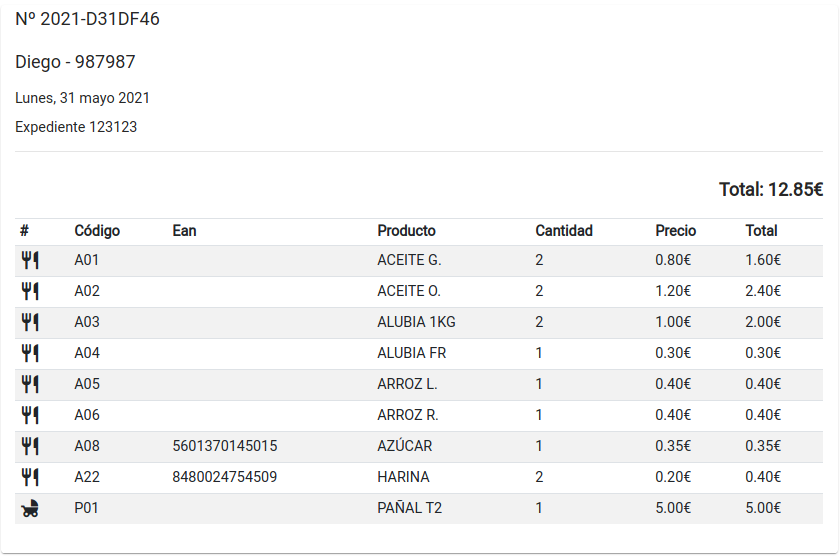
\includegraphics[scale=0.47]{archivos/maquetacion-factura.png}
\caption{Pedidos: Vista previa factura}
\label{fig:pedidos_invoice_preview}
\end{figure}
\clearpage
\begin{figure}[h]
\centering
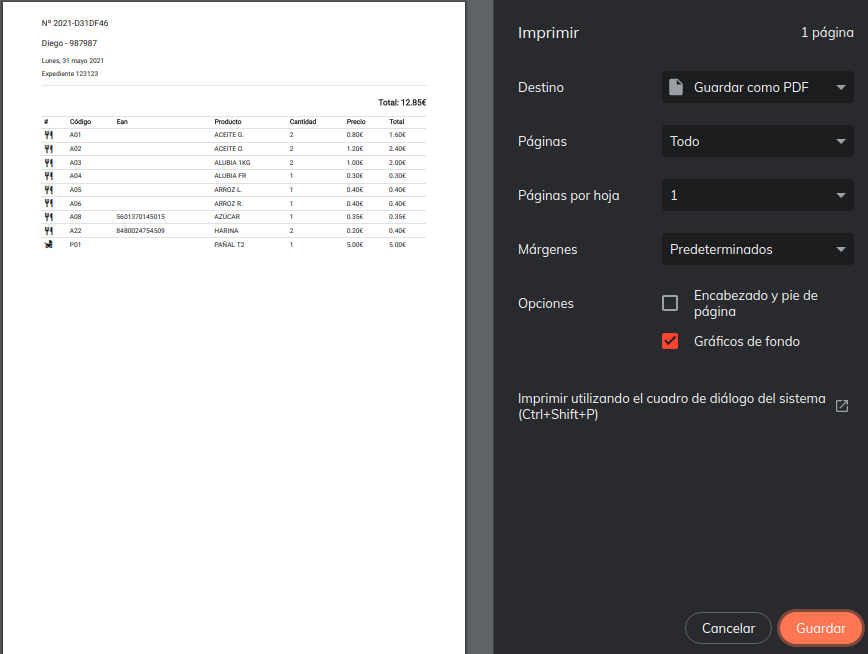
\includegraphics[scale=0.47]{archivos/imprimir-factura.png}
\caption{Pedidos: Imprimir factura}
\label{fig:pedidos_invoice_print}
\end{figure}
\clearpage
\subsection{Caja}
La sección de caja es un conjunto de acordeones que se complementan entre sí para mostrar las facturas abiertas, cobradas y cerradas (anuladas) y, por último, un resumen de caja.
\vspace{1em}
\par Las facturas que se muestra, por defecto son del día en curso, pero se puede cambiar el rango de fechas para consultar otras facturas. Además, en caso de que el usuario sea administrador, éste podrá anonimizar las facturas que se estén incluidas en el rango de fechas especificado.

\begin{figure}[h]
\centering
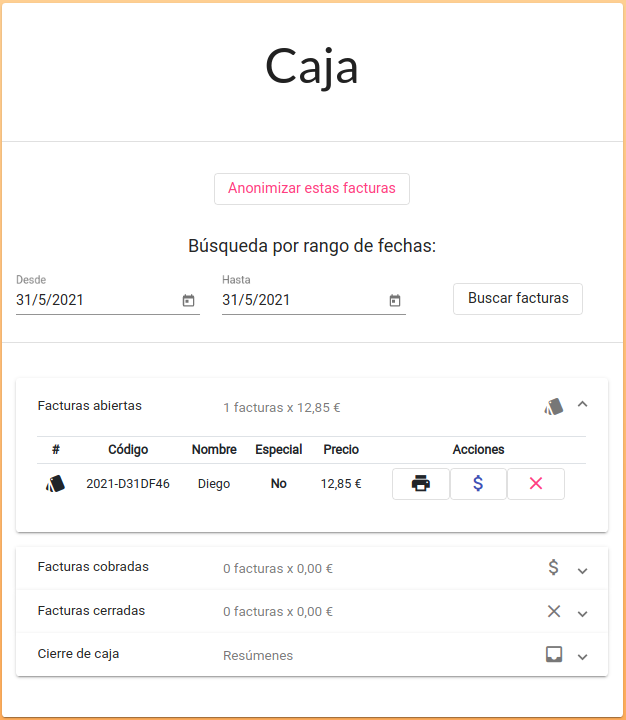
\includegraphics[scale=0.47]{archivos/caja.png}
\caption{Caja}
\label{fig:caja}
\end{figure}
\clearpage

\subsection{Almacén}
La sección de almacén es un conjunto de acordeones que se complementan entre sí para mostrar los pedidos sin despachar.
\vspace{1em}
\par Cuando se quiere despachar un pedido, aparecerá un listado de sus productos con la capacidad de marcarlos para saber si se ha preparado ya o no, esta funcionalidad se ha realizado a petición expresa de voluntarios de almacén del banco de alimentos al que se entregará el proyecto.

\begin{figure}[h]
\centering
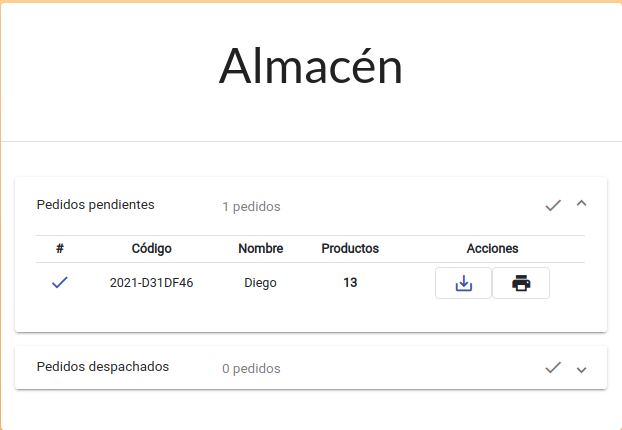
\includegraphics[scale=0.5]{archivos/almacen_1.png}
\caption{Almacén - Resumen de pedidos por despachar}
\label{fig:almacen_resumen}
\end{figure}

\begin{figure}[h]
\centering
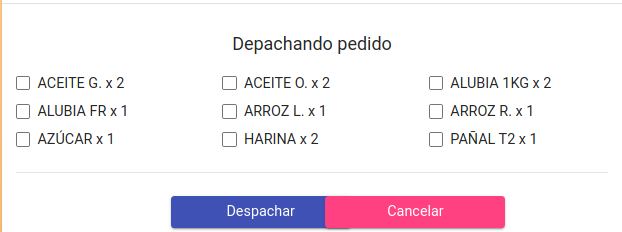
\includegraphics[scale=0.5]{archivos/almacen_2.png}
\caption{Almacén - Despachando un pedido}
\label{fig:almacen_despachando}
\end{figure}
\clearpage

\section{Implementación}
En este apartado se detallarán implementaciones que tengan relevancia en el desarrollo del proyecto, dándole un trasfondo y sentido a las pantallas que se acaban de mostrar.

\subsection{Base de datos}
Para la realización de este proyecto se ha decidido trabajar con una base de datos no relacional, en concreto con MongoDB que es una base de datos basada en documentos. Usar MongoDB como motor de base de datos ha venido especialmente bien al proyecto pues, además de usar JSON como esquema base de los documentos, hemos podido usar Compass y su capa gratuita de cluster en la nube.

\begin{lstlisting}[caption={Inyección proveedores ddbb},label=cod:ddbb-providers-injection]
export const databaseProviders = [
  {
    provide: 'MONGODB_CONNECTION',
    imports: [ConfigModule],
    inject: [ConfigService, Logger],
    useFactory: (
      configService: ConfigService<AppConfig>,
      logger: LoggerService,
    ): Promise<typeof mongoose> => {
      logger.log('CONNECTION MADE', 'ProvidersModule');
      return mongoose.connect(configService.get('mongoUrl'), {
        useNewUrlParser: true,
        useUnifiedTopology: true,
      });
    },
  },
];
\end{lstlisting}
\vspace{1em}
\par Dado que para el buen funcionamiento de la aplicación nos había solicitado atomizar los permisos que tiene cada usuario para acceder a los datos, se decidió hacer un mapa que incluye una relación entre el rol que se requiere y la lista de roles que podría tener el usuario para que el permiso fuese concedido. Por ejemplo, para realizar acciones de almacén, se debe tener cualquiera de los roles relacionados, que en esta caso son cualquiera de los 3 de administrador ó el propio de almacén. Este cruce se ideó con el pensamiento a futuro de que la aplicación pudiese crecer, complicarse los permisos y que hubiese algunos que colisionasen, por ejemplo, un permiso que fuese imprimir facturas y que éste fuese únicamente permitido a administradores, caja y pedidos; con esta implementación sólo habría que añadir un nuevo elemento al mapa con los permisos permitidos y toda la aplicación se vería afectada inmediatamente.
\clearpage
\begin{lstlisting}[caption={Gestión de roles para acceder a datos},label=cod:ddbb-roles]
export class Role {
  static permissionMap: RolePermissionMap;
  static initPermissionMap(): void {
    const map = new Map<RoleName, RoleName[]>();
    map.set(RoleName.SUPERADMIN, [RoleName.SUPERADMIN]);
    map.set(RoleName.ADMIN, [RoleName.SUPERADMIN, RoleName.ADMIN]);
    map.set(RoleName.ADMINLOCAL, [
      RoleName.SUPERADMIN,
      RoleName.ADMIN,
      RoleName.ADMINLOCAL,
    ]);
    map.set(RoleName.ALMACEN, [
      RoleName.SUPERADMIN,
      RoleName.ADMIN,
      RoleName.ADMINLOCAL,
      RoleName.ALMACEN,
    ]);
    map.set(RoleName.RECEPCION, [
      RoleName.SUPERADMIN,
      RoleName.ADMIN,
      RoleName.ADMINLOCAL,
      RoleName.RECEPCION,
    ]);
    map.set(RoleName.FAMILIAR, [
      RoleName.SUPERADMIN,
      RoleName.ADMIN,
      RoleName.ADMINLOCAL,
      RoleName.FAMILIAR,
    ]);
    map.set(RoleName.CAJA, [
      RoleName.SUPERADMIN,
      RoleName.ADMIN,
      RoleName.ADMINLOCAL,
      RoleName.CAJA,
    ]);
    Role.permissionMap = map;
  }
  static hasNeededRole(input: RoleName[], needed: RoleName): boolean {
    if (!Role.permissionMap) {
      Role.initPermissionMap();
    }
    const allowed = Role.permissionMap.get(needed);
    return allowed && input.some((role) => allowed.includes(role));
  }
}
\end{lstlisting}
\clearpage

\subsection{Esquemas y servicios}
\subsubsection{Login y registro}
\begin{lstlisting}[caption={User schema},label=cod:ddbb-user-schema]
export type UserDocument = User & Document;

export class UserComment {
  @Prop() author: string;
  @Prop() comment: string;
}

export class UserAction {
  @Prop() date: Date;
  @Prop() action: string;
}

@Schema()
export class User {
  @Prop() name: string;
  @Prop() email: string;
  @Prop() password: string;
  @Prop() active: boolean;
  @Prop() permissions: RoleName[];
  @Prop() warehouses: string[];
  @Prop() accessHistory: Date[];
  @Prop() actionsHistory: UserAction[];
  @Prop() comments: UserComment[];

  constructor(o: User) {
    Object.assign(this, o);
  }

  static fromUserDto(user: UserDto): User {
    return new User({
      name: user.name,
      email: user.email,
      active: user.active,
      permissions: user.permissions.map((p: RoleName) => p),
      warehouses: user.warehouses.map((w: string) => w),
      accessHistory: user.accessHistory.map((h: string) => new Date(h)),
      actionsHistory: user.actionsHistory.map((h: UserActionDto) => ({
        action: h.action,
        date: new Date(h.date),
      })),
      comments: user.comments.map((c: UserCommentDto) => ({
        author: c.author,
        comment: c.comment,
      })),
    });
  }
}

export const UserSchema = SchemaFactory.createForClass(User);
\end{lstlisting}

\vspace{1em}
\par El documento usuario contiene su propia contraseña, la cual está resumida con bcrypt y 10 rondas, veamos cómo se crea un usuario y cómo se hace login:
\vspace{1em}
\par 
\begin{lstlisting}[caption={Creación de un usuario},label=cod:service-user-creation]
@Injectable()
export class UserService {
  private hashRounds = 10;

  async createUser(input: UserDto): Promise<UserDto> {
    this.userValidations(input);
    const repeated: UserDocument = await this.userMongo.findOneBy(
      'email',
      input.email,
    );
    if (repeated)
      throw new ConflictException(`The email ${input.email} is in use`);
    input.password = hashSync(input.password, this.hashRounds);
    const user = User.fromUserDto(input);
    return UserService.userMapper(await this.userMongo.create(user));
  }
}
\end{lstlisting}
\vspace{1em}
\par 
\begin{lstlisting}[caption={Login de un usuario},label=cod:service-user-login]
@Injectable()
export class LoginService {
  private genericErrorMessage = 'Login error';

  async login(input: LoginDto): Promise<UserDto> {
    const user = (await this.userMongo.findBy('email', input.email))[0];
    if (!user) throw new ForbiddenException(this.genericErrorMessage);
    if (!compareSync(input.password, user.password))
      throw new ForbiddenException(this.genericErrorMessage);
    if (!user.active) {
      user.actionsHistory.push({
        date: new Date(),
        action: 'Attempt to login when inactive',
      });
      await user.save();
      throw new ForbiddenException(this.genericErrorMessage);
    }
    user.accessHistory.push(new Date());
    await user.save();
    return UserService.userMapper(user);
  }
}
\end{lstlisting}
\vspace{1em}
\par El mapeo de salida de un usuario limpia datos sensibles, en este caso es exclusivamente la contraseña.
\clearpage

\subsubsection{Productos}
El documento de productos contiene los datos necesarios para identificarlos correctamente, además de aquellos datos relacionados con OpenFoodFacts. Cada producto está relacionado con su almacén, por lo que almacenes con el mismo producto tendrán duplicidad de datos, algunos innecesarios, como los nutricionales. Una posible mejora sería sacar datos nutricionales a una colección distinta y relacionarlos por ean para evitar duplicidad, como ahora mismo sólo se tiene vista a usar un único almacén, ésta implementación se decidió dejar para versiones posteriores.
\vspace{1em}
\par 
\begin{lstlisting}[caption={Esquema de producto},label=cod:ddbb-product-schema]
export type ProductDocument = Product & Document;

export class ProductLimits {
  @Prop() price: number;
  @Prop() quantity: number;
}

@Schema()
export class Product {
  @Prop() ean: string;
  @Prop() name: string;
  @Prop() alias: string;
  @Prop() quantity: string; // amount or weight
  @Prop() categories: string;
  @Prop() ingredients: string;
  @Prop() allergens: string;
  @Prop() labels: string;
  @Prop() imageUrl: string;
  @Prop() limits: ProductLimits[];
  @Prop() pvp: number;
  @Prop() code: string; // Inner code for every warehouse
  @Prop() type: string;
  @Prop() chargeableOutBudget: boolean;
  @Prop() warehouse: string;

  constructor(o: Product) {
    Object.assign(this, o);
  }
}

export const ProductSchema = SchemaFactory.createForClass(Product);
\end{lstlisting}
\clearpage
\vspace{1em}
\par Veamos cómo se crea un producto y, en caso de tener EAN, se consulta con el api pública de OpenFoodFacts para recuperar los datos nutricionales de éste.
\begin{lstlisting}[caption={Product service: Añadir producto nuevo},label=cod:service-product-create-product]
@Injectable()
export class ProductService {
  private openFoodUrl =
    'https://world.openfoodfacts.org/api/v0/product/{{ean}}.json';
  async create(
    input: CreateProductResponseDto,
  ): Promise<ReadProductResponseDto> {
    let product = {} as Product;
    product.alias = input.alias;
    product.limits = input.limits;
    product.pvp = input.pvp;
    product.code = input.code;
    product.type = input.type;
    product.chargeableOutBudget = input.chargeableOutBudget;
    product.ean = input.ean;
    let openFoodResponse = {};
    if (product.ean)
        openFoodResponse = await this.readByEan(product.ean);
    product = {
      ...ProductService.fromOpenFoodToProduct(openFoodResponse),
      ...product,
    };
    return ReadProductResponseDto.fromProductDocument(
      await this.productsMongo.create(product),
    );
  }
  async readByEan(ean: string): Promise<any> {
    const response: AxiosResponse = await this.httpClient
      .get(this.openFoodUrl.replace('{{ean}}', ean), {
        headers: { 'User-Agent': this.config.get('openFoodUserAgent') },
      }).toPromise();
    if (!response.data.product)
      throw new InternalServerErrorException('Error requesting to openfood');
    return response.data.product;
  }
  private static fromOpenFoodToProduct(response: any): Product {
    return {
      name: response.product_name_es || response.product_name,
      ean: response.code,
      quantity: response.quantity,
      categories: response.categories,
      labels: response.labels,
      allergens: response.allergens,
      ingredients: response.ingredients_text_es || response.ingredients_text,
      imageUrl: response.image_front_url,
    } as Product;
  }
}
\end{lstlisting}
\clearpage

\subsubsection{Pedidos}
El documento de pedidos contiene los datos que hacen falta para dar completa funcionalidad a lo que se nos pidió que era necesario para procesar los pedidos de las familias.
\vspace{1em}
\par Una de las claves, es que aparecen varios identificadores de usuario, dado que es un sistema muy centrado en permitir quién puede hacer qué, es necesario almacenar quién ha hecho qué; en este caso, quién ha creado el pedido, quién lo ha cobrado y quién lo ha despachado, además de cuándo se han realizado estas acciones.
\vspace{1em}
\par Dado que la información sobre las familias está almacenada, mantenida y expedida por Cáritas, en este documento se relaciona el pedido con el documento identificativo de la familia y su expediente de Cáritas, no almacenamos datos de ningún tipo en ninguna otra colección, dado que no se sabía si tendríamos permiso, además, no resulta necesario para dar ninguno de los servicios propuestos. Esta forma de relacionar cada pedido con la familia origen, facilitó la búsqueda de qué familias han hecho visitas el mes en curso (por las restricciones) y, además, la anonimización de los pedidos, pues únicamente hay que vaciar esos campos en los pedidos del rango de fechas que se especifica en la llamada.
\vspace{1em}
\par Uno de los quebraderos de cabeza que se tuvo en el proyecto hasta llegar a este esquema final, fue que en principio se quería restringir los pedidos cuando las familias ya habían superado sus límites, pero en las reuniones de sprint en el economato llegamos a saber que habían problemas de colisión entre expedientes y documentos de identificación, que debían resolver personalmente llamando por teléfono a la sede de Cáritas. Por lo que acabamos haciendo el sistema flexible a las colisiones en este sentido y, si se revisan los vídeo-tutoriales adjuntos, se podrá apreciar que en caso de una colisión es el voluntario el que puede decidir manualmente si esta colisión afecta o no a los límites que impone el sistema.
\vspace{1em}
\par Además de lo anterior, dado que las órdenes es algo que se está consultando continuamente por diferentes secciones de la aplicación, se incluyó caché en la misma aplicación, de ésta forma salvo que la lista de pedidos del día corriente cambie, siempre que se consulten se devolverá el caché en lugar de acceder a base de datos. De ésta forma ahorramos ancho de banda y, si fuese una capa de pago, coste por procesamiento y transferencia de las consultas innecesarias.
\vspace{1em}
\par Estas peticiones tan repetitivas fue sacada a la luz por una necesidad que apareció conforme iba creciendo la aplicación, hay diferentes pantallas desde donde se está esperando que el listado de pedidos se actualice y, además, pueden ser diferentes personas/dispositivos las que estén a espensas de estos cambios. Así, pues, se hizo uso de la tecnología de websockets para poder comunicar en tiempo real cambios en los pedidos, ya sea una adición nueva, un cobro, una cancelación o haberlo despachado. Si se revisan los vídeo-tutoriales adjuntos se podrá apreciar cómo un usuario recibe en tiempo real los cambios ejecutados por otro en otro navegador.
\clearpage
Veamos el esquema de los pedidos:
\begin{lstlisting}[caption={Esquema de pedido},label=cod:ddbb-order-schema]
export type OrderDocument = Order & Document;

export class ProductResume {
  @Prop() id: string;
  @Prop() ean: string;
  @Prop() code: string;
  @Prop() name: string;
  @Prop() amount: number;
  @Prop() pvp: number;
}

@Schema({ strict: false })
export class Order {
  @Prop({ index: true }) code: string; // Code for easy human identification
  @Prop() headquarter: string; // foreign key headquarter collection
  @Prop() familyName: string;
  @Prop({ index: true }) expedient: string;
  @Prop({ index: true }) credential: string;
  @Prop() special: boolean;
  @Prop() products: ProductResume[]; // list of products
  @Prop() pvp: number;
  @Prop() type: string;
  @Prop() chargeableOutBudgetSelected: boolean;
  @Prop() createdAt: Date;
  @Prop() updatedAt: Date;
  @Prop() paid: boolean;
  @Prop() deleted: boolean;
  @Prop() origin: string; // USER ID
  @Prop() resolver: string; // USER ID
  @Prop() resolvedAt: Date;
  @Prop() dispatcher: string; // USER ID
  @Prop() dispatched: boolean;
  @Prop() dispatchedAt: Date;
}

export const OrderSchema = SchemaFactory.createForClass(Order);
\end{lstlisting}
\clearpage
\vspace{1em}
\par La creación de pedidos es una de las implementaciones que hace uso de los websockets, pues hay secciones de la aplicación que deben actualizarse en tiempo real cuando aparecen nuevos datos. Veamos cómo se ha resuelto esto:
\begin{lstlisting}[caption={Invoice service: Crear nuevo pedido},label=cod:service-invoice-create-order]
@Injectable()
export class InvoiceService {
  async create(input: Order, jwt: JWToken): Promise<any> {
    input.createdAt = new Date();
    input.updatedAt = new Date();
    input.code = `${new Date().getFullYear().toString()}-${uid(7).toUpperCase()}`;
    input.paid = false;
    input.deleted = false;
    input.origin = jwt.id;
    const order: OrderDocument = await this.mongo.create(input);
    this.broadcastInvoiceResolved(order.id, ResolveInvoiceAction.CREATED);
    await this.saveUserAction(jwt,`Invoice ${order.id} created by ${order.id}`,);
    await this.refreshCache();
    return order.toObject();
  }
  private broadcastInvoiceResolved(
    invoiceId: string,
    action: ResolveInvoiceAction,
  ): void {
    this.wsService.broadcastInvoice({ invoiceId, action });
  }
}
\end{lstlisting}
\begin{lstlisting}[caption={Websocket service: Difusión de mensajes},label=cod:service-websocket-broadcast]
@Injectable()
@WebSocketGateway()
export class WebsocketsService
  implements OnGatewayConnection, OnGatewayDisconnect {
  private wsClients: any[] = [];
  broadcastInvoice(message: InvoiceMessage): void {
    const data: WsInvoiceMessage = { event: WsTopics.INVOICES, data: message };
    this.broadcast(data, { id: null } as Socket);
  }
  broadcast(message: WsMessage | string, sender: Socket): void {
    const payload: WsMessage = { event: WsTopics.UNKNOWN, data: '' };
    if (typeof message === 'string') payload.data = message;
    else {
      payload.event = message.event;
      payload.data = message.data;
    }
    for (const c of this.wsClients) {
      if (c.id === sender.id) return;
      c.send(JSON.stringify(payload));
    }
  }
}
\end{lstlisting}
\clearpage

\subsubsection{Caja}
La gestión de caja hace uso del documento de pedidos, editando lo que necesita para dar funcionalidad a lo solicitado.
\vspace{1em}
\par Recordemos que la caja debe permitir dos acciones, cobrar pedidos o cerrarlos por erróneos. Ésto afectará al listado de pedidos del día corriente, por lo que debe actualizar la caché y, además, difundir el mensaje por websocket para que todos los clientes sepan que ha habido un cambio.
\vspace{1em}
\par Ésta implementación es susceptible de mejora, ahora mismo cuando el servidor cambia un pedido, actualiza la caché y avisa por difusión a los clientes de que ha habido un cambio, esto provoca que inmediatamente haya un aluvión de solicitudes para recuperar la lista de pedidos actualizada. Dado que está cacheada, el servidor tan cual recibe la solicitud despacha los datos directamente de la ram, sin pasar por base de datos, pero aún así, es ineficiente; sobretodo si hay muchos clientes conectados. La mejora podría consistir en difundir el nuevo estado del pedido con su identificador, de ésta forma, los clientes pueden actualizar ese pedido en concreto en sus datos locales sin más. Dado que todo lo relacionado con esta funcionalidad no era una necesidad y se hizo como mejora, se decidió que este último punto se delegase a versiones futuras, ya que impactaría en la forma en la que se difunden los mensajes y en la que los clientes deciden qué hacer con éstos.
\clearpage
Veamos la sección de código en la que se cambia el estado de un pedido de pendiente a cobrado/cerrado:
\vspace{1em}
\par 
\begin{lstlisting}[caption={Invoice service: Resolver pedido},label=cod:service-invoice-resolve-order]
export enum ResolveInvoiceAction {
  CLOSE,
  PAY,
  CREATED,
}
@Injectable()
export class InvoiceService {
  async resolveInvoice(
    id: string,
    action: ResolveInvoiceAction,
    jwt: JWToken,
  ): Promise<void> {
    const order: OrderDocument = await this.mongo.findById(id);
    if (!order) throw new NotFoundException(`Invoice with id ${id} not found`);
    if (order.paid || order.deleted) {
      throw new PreconditionFailedException('This invoice is already resolved');
    }
    switch (action) {
      case ResolveInvoiceAction.CLOSE:
        order.deleted = true;
        break;
      case ResolveInvoiceAction.PAY:
        order.paid = true;
        break;
      default:
        throw new InternalServerErrorException('Action against invoice not implemented');
    }
    this.broadcastInvoiceResolved(id, action);
    order.updatedAt = new Date();
    order.resolvedAt = new Date();
    order.resolver = jwt.id;
    await order.save();
    await this.saveUserAction(
      jwt,
      `Invoice ${order.id} updated by ${jwt.id} with action ${action}`,
    );
    await this.refreshCache();
  }
}
\end{lstlisting}
\clearpage

\subsubsection{Almacén}
La gestión de almacén también hace uso del documento de pedidos, editando lo que necesita para dar funcionalidad a lo solicitado.
\vspace{1em}
\par De una forma similar a la caja, el almacén tiene una funcionalidad muy concreta, ésta es despachar pedidos y nada más. Como bien se estuvo comentando antes, esto cambia el listado de órdenes del día y refrescará caché además de difundir el mensaje por websocket.
\vspace{1em}
\par 
\begin{lstlisting}[caption={Invoice service: Despachar pedido},label=cod:service-invoice-dispatch-order]
@Injectable()
export class InvoiceService {
  async dispatchOrder(id: string, jwt: JWToken): Promise<OrderDocument> {
    const order: OrderDocument = await this.mongo.findById(id);
    if (!order) throw new NotFoundException(`Invoice with id ${id} not found`);
    if (order.dispatched)
      throw new PreconditionFailedException('This order has been dispached already');
    order.dispatched = true;
    order.dispatcher = jwt.id;
    order.dispatchedAt = new Date();
    order.updatedAt = new Date();
    await order.save();
    await this.saveUserAction(jwt, `Order ${order.id} dispatched by ${jwt.id}`);
    this.deleteCache();
    return order;
  }
}
\end{lstlisting}
\clearpage

\subsubsection{Roles y controladores}
Por último, se procede a explicar cómo se han implementado la salvaguarda de roles en Nestjs, y dónde y cómo afecta a la aplicación.
\vspace{1em}
\par Como ya se ha comentado, uno de los requisitos indispensables es la gestión de roles de forma atómica, con solape o sin él, para manejar los permisos de los usuarios lo más estrictamente posible. De esta forma, se optó por un patrón de seguridad que se inició en los sistemas linux y se puso muy de moda en la gestión de usuarios en los servicios de infraestructura cloud. Éste es el del permiso más restrictivo por defecto, es decir, no se tendrá acceso a no ser que explícitamente se diga lo contrario.
\vspace{1em}
\par Para poder simular este patrón en el proyecto, hicimos 2 implementaciones haciendo uso del patrón Guard de Nestjs, éste viene a ser un servicio que se ejecuta antes de cualquier solicitud y que decide si se tiene acceso o no a ese recurso. Para este proyecto hay 2 guards, haciendo su magia respectivamente, en función de:
\begin{itemize}
    \item Token Bearer con un Json Web Token
    \item Roles permitidos en la ruta
\end{itemize}
\vspace{1em}
\par Su uso en Nestjs sería el siguiente:
\begin{lstlisting}[caption={User Controller: Guards en el controlador de usuario},label=cod:controller-user-guards]
@Controller('user')
@UseGuards(JwtGuard, RolesGuard)
export class UserController {
  constructor(private service: UserService) {}
  
  @Get('/:id')
  @Roles(RoleName.OWNER, RoleName.ADMINLOCAL)
  async readUserById(@Param('id') id: string): Promise<UserDto> {
    const result: UserDto = await this.service.readUserById(id);
    return result;
  }
}
\end{lstlisting}
\vspace{1em}
\par Mediante estos decoradores damos lógica automáticamente a esta clase, se convierte en un controlador de la ruta '/user' para el servidor web en Express, hace uso a nivel de controlador de los 2 guards y, en la ruta '/:id', escribe expresamente qué roles son necesarios para acceder a esa ruta.
\clearpage
El orden de los guards es importante, primero se debe manejar el jwt ya que ahí está incluído el identificador del usuario y, entre otros datos, su lista de permisos.
\begin{lstlisting}[caption={Guard JWT: Verificación de un json web token e inyección de datos en la request},label=cod:guard-jwt]
@Injectable()
export class JwtGuard implements CanActivate {
  constructor(private configService: ConfigService<AppConfig>) {}
  canActivate(context: ExecutionContext): Promise<boolean> {
    const req: Request = context.switchToHttp().getRequest();
    const bearer: string = req.header('Authorization');
    let token: JWToken;
    try {
      const regex = /^bearer (.+)$/i;
      const g = regex.exec(bearer);
      token = jwt.verify(g[1], this.configService.get('jwtSecret'));
    } catch (err) {
      throw new UnauthorizedException('Bad bearer token');
    }
    req['jwt'] = token;
    return true;
  }
}
\end{lstlisting}
\vspace{1em}
\par Este guard por defecto siempre devuelve true, ya que el único caso en el que debería impedir pasar es cuando el jwt no se puede verificar (no coincide el secreto de la firma o ha caducado), caso en el que se lanza una excepción más intuitiva. Dado que los datos extraídos del jwt deber ser accesibles más adelante, es común en Express pasar información entre middlewares inyectándolos directamente en la request, tal y como se hace en la línea 15 del código \ref{cod:guard-jwt}.
\vspace{1em}
\par Una vez verificada la identidad del usuario, se procede a revisar su rol, pasando por la implementación del guard de roles:
\begin{lstlisting}[caption={Guard Roles: Verificación de roles necesarios para el acceso},label=cod:guard-roles]
@Injectable()
export class RolesGuard implements CanActivate {
  constructor(private reflector: Reflector) {}
  canActivate(context: ExecutionContext): boolean {
    const roles = this.reflector.get<RoleName[]>('roles', context.getHandler());
    if (!roles) throw new InternalServerErrorException('Roles needed in route');
    const req: Request = context.switchToHttp().getRequest();
    const token: JWToken = req['jwt'];
    if (roles.includes(RoleName.OWNER)) {
      if (roles.length === 1) return req.params.id === token.id;
      if (req.params.id === token.id) return true;
    }
    return roles
      .filter((role) => role !== RoleName.OWNER)
      .some((role) => Role.hasNeededRole(token.roles, role));
  }
}
\end{lstlisting}
\clearpage
Esta implementación nos indica lo siguiente del guard de roles:
\begin{itemize}
    \item Es completamente obligatorio que la ruta que está siendo solicitada tenga el decorador de roles asignado.
    \begin{itemize}
        \item Línea 6 del código \ref{cod:guard-roles}
    \end{itemize}
    \item Si la ruta tiene un rol y es exclusivamente OWNER, no es cuestión de rol si no de ser dueño de los datos, si no se da el caso se corta el acceso.
    \begin{itemize}
        \item Línea 10 a 13 del código \ref{cod:guard-roles}
    \end{itemize}
    \item Por último, se verifica que de los roles que tiene el usuario, haya al menos uno compatible con las necesidades de la ruta.
    \begin{itemize}
        \item Línea 14 a 16 del código \ref{cod:guard-roles}
    \end{itemize}
\end{itemize}
\vspace{1em}
\par De esta forma tenemos las rutas protegidas, primero, obligando a que haya que acreditarse siempre; y segundo, obligando a que el desarrollador explícitamente indique qué permisos se deben complacer en las rutas que expone en la aplicación.
\vspace{1em}
\par A esta implementación le hace falta una mejora, ésta consistiría en asegurarse de poder hacer caducar los tokens, ahora mismo estos caducan a las 8 horas de su creación, para facilitar el trabajo de los voluntarios y no tener que estar logueando durante la jornada. El problema de ésto es que no se le puede retirar el acceso a alguien sin ir a su dispositivo a cerrar la sesión, habría que esperar a que le caduque el token.
\vspace{1em}
\par Veamos cómo se crean los tokens en el login de los usuarios:
\vspace{1em}
\par
\begin{lstlisting}[caption={Jwt service: Creación de token},label=cod:service-jwt-create]
createJwt(user: UserDto): string {
  const secret = this.configService.get('jwtSecret');
  const payload: Partial<JWToken> = {
    id: user.id,
    exp: moment().add(8, 'h').toDate().getTime(),
    roles: user.permissions,
    warehouses: user.warehouses,
  };
  return jwt.sign(payload, secret);
}
\end{lstlisting}
\clearpage

\section{Conclusiones, patrones y revisión del código}
Para terminar esta subsección, se procede a un pequeño análisis del código desarrollado, patrones utilizados y el framework elegido para mejorar la productividad.
\vspace{1em}
\par El uso del framework Nestjs ha permitido usar diferentes patrones de forma intuitiva y sin apenas codificar.
\begin{itemize}
    \item Patrón MVC clásico, con la salvedad de que la vista es mapeo e impresión de datos en json.
    \item Inyección de dependencias, Nestjs permite una configuración de módulos muy intuitiva que permite inyectar dependencias en el constructor de las clases con muy poca configuración, de esta forma la inicialización de las clases de las que depende la lógica de negocio es completamente agnóstica a la misma lógica de negocio.
    \item Patrón singleton, los servicios injectables en Nestjs que se importan desde módulos independientes tienen la peculiaridad de que sólo se instancian una vez por módulo, ahorrando memoria y errores de implementación en caso de querer hacerlo manualmente.
    \item Patrón factory, Nestjs usa una factory por defecto para crear el model de Mongodb a partir de una clase decorada como esquema. Además, en el proyecto se ha usado el patrón factory para construir los dto de salida a partir de un documento de Mongodb.
\end{itemize}
\vspace{1em}
\par Nestjs tiene muchos más beneficios, como el enrutado automático del servidor web o la configuración automática del servidor de documentación basado en swagger.
\vspace{1em}
\par Para el frontend se ha usado Angular 11, del cual se ha expuesto menos código ya que es muy similar al backend. Ésta fue una de las razones de usar la combinación Nestjs y Angular, ambos son MVC con módulos configurables e inyectables y usan una sintaxis muy similar, de ésta forma ser conocedor de uno de los dos framework hace el acercamiento al otro mucho más sencillo y con muy poca curva de aprendizaje.
\vspace{1em}
\par Para ahorrar esfuerzo y tiempo en diseño se han usado paquetes de Angular que traen animaciones y maquetaciones, Angular Material. Y para la estructuración y el responsive se ha usado Bootstrap 4, éste no es de Angular pero hay integraciones libres de la comunidad que integran a la perfección las dependencias de Bootstrap con las de Angular para hacer funcionar sin problema este framework.
\clearpage
Más allá de los frameworks, en el desarrollo del backend se ha hecho especial hincapié en desarrollar teniendo en mente los principios SOLID \citep{SOLID}:
\begin{itemize}
    \item S: Responsabilidad única.
    \begin{itemize}
        \item División del proyecto en módulos y servicios independientes, intentando siempre que cada clase y/o función se haga cargo exclusivamente de lo que le concierne.
    \end{itemize}
    \item O: Principio abierto/cerrado.
    \begin{itemize}
        \item Cuando se ha tenido que añadir o cambiar lógica, se ha intentado siempre minimizar el impacto que esto tiene sobre las funcionalidad actuales. Las factories han servido de ayuda, ya que aíslan funcionalidades concretas de forma estática e independiente de clases relacionadas. 
    \end{itemize}
    \item L: Sustitución de Liskov.
    \begin{itemize}
        \item Cuando hay herencia, las clases hijas deben servir para lo mismo que para los padres. En este proyecto se ha usado herencia de una clase abstracta para dar funcionalidad genérica a servicios de la capa de datos, las funcionalidad no cambian entre servicios, sólo las colecciones a las que hacen referencia.
    \end{itemize}
    \item I: Segregación de interfaces.
    \begin{itemize}
        \item Se ha intentado hacer prevalecer la alta cohesión frente al acoplamiento, la modularización de Nestjs ha ayudado en este menester.
    \end{itemize}
    \item D: Inversión de dependencias
    \begin{itemize}
        \item Principalmente en la capa de acceso a datos, se ha implementado de forma que los detalles dependen de las abstracciones y no al revés.
    \end{itemize}
\end{itemize}
\vspace{1em}
\par Para finalizar, se ha pretendido mantener el código todo lo seco posible: DRY (Don't Repeat Yourself), haciendo uso de herencias, funciones y extrayendo a módulos inyectables las codificaciones que se han detectado como generalizaciones.

\section{Resultado final}
Para finalizar este capítulo sabe señalar que hay mucho más código y muchos más detalles en la aplicacíon de lo que se puede expresar en un documento. Por lo que se va a aprovechar este cierre para incluir enlaces directamente a los servicios desplegados en producción, vídeo-tutoriales que se han entregado junto al proyecto al economato social y el enlace al proyecto en el repositorio remoto Github.
\begin{itemize}
    \item \href{https://economato-social-api.herokuapp.com}{Enlace al Backend} \citep{BACKEND}
    \item \href{ttps://economato-social.herokuapp.com}{Enlace al Frontend} \citep{FRONTEND}
    \item \href{https://github.com/DiegoMGar/TFG}{Enlace al Repositorio público en Github}  \citep{REPOSITORIO}
    \item \href{https://drive.google.com/drive/folders/1pv-6iishQkM29StiSHUyY74lWEVx0t6q}{Enlace a los Vídeo-tutoriales} \citep{VIDEOTUTORIALES}
\end{itemize}
